
\chapter{Orlin's Algorithm} \label{chap:Orlin}

    Before delving into Orlin's algorithm, let's review the current state of the problem.  
    The Goldberg-Rao algorithm achieves what is called a \textit{weakly polynomial} time complexity, solving the problem in \(\log mU\) phases, each with a cost of \( O(\Lambda m \log(n^2/m)) \), where \( \Lambda = \min \{n^{2/3}, m^{1/2}\} \).  
    If we aim to solve the maximum flow problem with a \textit{strongly polynomial} time complexity, there is the King-Rao-Tarjan algorithm. However, this algorithm achieves a time cost of \( O(nm) \) only under the condition that \( m = \Omega (n^{1+\varepsilon}) \) for some \( \varepsilon > 0 \).  
    If the number of edges is insufficient, its cost is \( O(nm \log_{m / (n \log n)} n) \).  

    In the following algorithm, James B. Orlin proposes a solution that, by leveraging the Goldberg-Rao algorithm, manages to solve the maximum flow problem in \( O(nm) \) when \( m = O(n^{1+\varepsilon}) \). This makes it possible to solve the problem in strictly polynomial time for any values of \( n \) and \( m \), without being limited by edge capacities.


\section{Idea}

    The idea arises from several observations:\\
    The Goldberg-Rao algorithm operates through \textbf{increment phases} that take a \(\Delta\)-optimal flow and make it \(\Delta/2\)-optimal.  
    Furthermore, it is noted that \(\log_{8m} mU \leq 1 + \log U\); in fact, from now on, \(\log U\) increment phases will be considered.  
    If we set \(\Lambda = O(m^{1/2})\), we can observe that  
    \[
    \log U < m^{7/16} \implies \tilde{O}(m^{3/2} \cdot m^{7/16}) = \tilde{O}(m^{31/16})
    \]
    (the notation \(\tilde{O}\) ignores logarithmic factors).\\
    Delving deeper into the calculations, we observe  
    \[
    \tilde{O}(m^{31/16}) = O(m \cdot m^{15/16} \cdot \log(n^2/m)) = O(m \cdot n^{(16/15)^{15/16}} \cdot \log(n^2/m))
    \]
    since we are looking for an algorithm when \(m = O(n^{1+\varepsilon})\). If \(1+\varepsilon < 16/15\) and \(\log U < m^{7/16}\), we can achieve an optimal solution with a polynomial cost of \(O(nm)\) by using only the Goldberg-Rao algorithm.

    However, this is only true if the number of edges is sufficiently larger compared to the edge with the maximum capacity.  
    
    Hence, the idea of contracting and compacting the network arises to ensure the calculation of the maximum flow under optimal conditions.

    The algorithm presents two bottlenecks:
    \begin{enumerate}
        \item Creation of the compacted representation (more precisely, maintaining the transitive closure)
        \item Transitioning from the compacted flow to the extended flow.
    \end{enumerate}

\section{Improvement phase}
If the Goldberg-Rao algorithm, in a sense, 'wraps' Dinic's Algorithm into a higher level of abstraction where the original graph is modified, Orlin does the same with Goldberg-Rao.

A higher level of increment phase is introduced, within which a slightly modified version of the Goldberg-Rao algorithm is executed.
So let's examine the input and output of each phase:

\begin{itemize}[itemsep=0.5ex]
    \item \textbf{Input}
    \begin{enumerate}
        \item a \textit{Flow} \(f\)
        \item a \textit{Residual Graph} \(G_f\), 
        \item an s-t cut \((S,T)\)
    \end{enumerate}
    Since with the flow and the residual graph, we can compose the residual function, when we consider the flow and the graph we can say to have also the residual function "r". \\
    We can represent the input as the tuple \((r, S, T)\).
    
    \item \textbf{Output}
    \begin{enumerate}
        \item a \textit{Flow} \(f'\)
        \item a \textit{Residual Graph} \(G_f'\)
        \item an s-t cut \((S', T')\) such that \(r'(S', T') \leq \frac{r(S, T)}{8m}\)
    \end{enumerate}
\end{itemize}

This phase is called the \(\Delta\text{-improvement phase}\), where \(\Delta = r(S, T)\). Alongside the parameter \(\Delta\), a parameter \(\Gamma\) is introduced, where \(\Gamma \leq \Delta\), which will be used to create the \(\Gamma\)-compact network.

Depending on the conditions, the \(\Delta\)-improvement will be executed either on the original network \(G\) or on the \(\Gamma\)-compact network \(G^c\), which we will introduce later.
\newpage

\section{$\Delta$-abundant e abundance graph}
In questa sezione viene presentato il concetto di \textbf{Abbondanza}.

\begin{definition}[$\Delta$-abundant arc]
    Let $\Delta = r(S,T)$ then any edge $(i,j)$ is said $\Delta$-abundant if $r_{ij} \ge 2\Delta$ 
     
\end{definition}
\begin{lemma}
    \label{ab4ever}
    Let $(r,S,T)$ be the input for a $\Delta\text{-}improvement\ phase$. If the edge  $(i,j)$ is abundant before the phase then it will be abundant for for all subsequent phases.
\end{lemma}
\begin{proof}
    Since
    $\Delta' \le \frac{\Delta}{8m} $ and recalling that $r_{ij} \ge 2\Delta $ it follows that 
    allora \[r'_{ij} \ge r_{ij}-\Delta \ge\Delta\ge  2\Delta'\]
\end{proof}

\begin{definition}[Abundance Graph]
    Given a network $G$, its \textbf{Abundance Graph} $G^{ab}$ is defined as: 
    \[G^{ab} := (N(G), \{(i,j)| (i,j)\in E(G)\land r_{ij}\ge 2\Delta\})\]
\end{definition}

\begin{obs}
    By lemma \ref{ab4ever}, as iterations proceed, the abundant graph can only acquire new edges, never lose them.
\end{obs}

The abundant graph has two purposes: 
\begin{enumerate}
    \item All cycles formed by abundant edges are \textit{contracted} into a single node.
    \item All nodes adjacent only to abundant edges (or edges with capacity that is too small) are \textit{compacted}.
\end{enumerate}

    Additionally, the algorithm maintains the transitive closure of all nodes connected by an \textbf{abundant path}, meaning a path composed only of abundant edges.\\
    If there exists an abundant path between nodes \( i \) and \( j \), this is indicated as \( i \implies j \), and the information is stored in an \textbf{M}$_{n \times n}$ matrix, where at position \textbf{M}$_{i,j}$ is the node that precedes \( j \) in the path starting from \( i \). If multiple paths are created during the iterations, the first one found is kept.

    The transitive closure can be maintained in time \( O(nm) \) using Italiano's algorithm\cite{ITALIANO1986273}. 
    In this way, it is always possible to reconstruct an abundant path \( P \) in \( O(|P|) \) (we will see later that contracting the graph does not prevent this nor does it alter its cost).

\newpage
\section{Contractions of abundant graph}
Let's now see how to exploit the abundant graph to contract the graph on which we calculate the max-flow and make the algorithm more efficient.

We analyze three different examples of contractions:

Suppose there are two nodes \(i\) and \(j\) such that \(r_{ij} \geq 2\Delta\) and \(r_{ji} \geq 2\Delta\).
We can contract the two nodes into a single one, preserving the edges of both.

\[\begin{tabular}{ccc}
    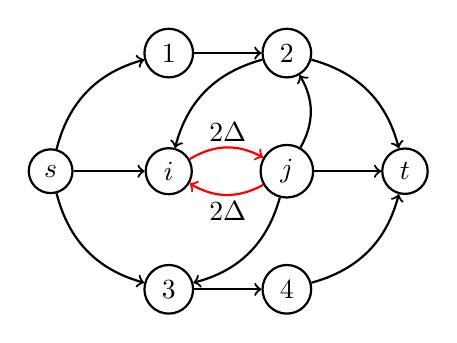
\begin{tikzpicture}[node distance={15mm}, thick , main/.style = {draw, circle}] 
    % Disegna i nodi del grafo
    

    \node[main] (0) {$s$};
    \node[main] (3) [right of= 0 ] {$i$};
    \node[main] (4) [right of=3] {$j$};
    \node[main] (1) [below of = 3 ] {3};
    \node[main] (2) [above of = 3] {$1$};
    
    \node[main] (6) [above of=4] {$2$};
    \node[main] (5) [below of=4] {$4$};
    \node[main] (7) [right of=4] {$t$};
    % Disegna gli archi orientati
    \draw[->] (0) [bend right] to (1);
    \draw[->] (0) [bend left] to (2);
    \draw[->] (0) to (3);
    \draw[->] (3) [red, bend left] to (4);
    \node at (2.25,0.5) {$2\Delta$};
    \node at (2.25,-0.5) {$2\Delta$};
    \draw[->] (4) [red, bend left] to (3);
    
    \draw[->] (2) to (6);
    \draw[->] (4)[bend left] to (1);
    \draw[->] (4)[bend right] to (6);
    \draw[->] (6)[bend right] to (3);
    \draw[->] (4) to (7);
    \draw[->] (1) to (5);
    \draw[->] (6)[bend left] to (7);
    \draw[->] (5)[bend right] to (7);


\end{tikzpicture}&\begin{tikzpicture}
    \node {$\implies$};% Freccia verso destra
    \node at (0,1.4) {};
    \node at (0,-1.6) {};
\end{tikzpicture}  &
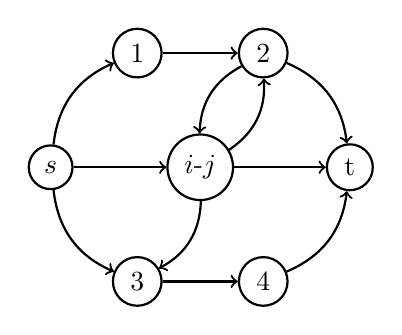
\begin{tikzpicture}[node distance={19mm}, thick , main/.style = {draw, circle}] 
    % Disegna i nodi del grafo
    
    
    \node[main] (m)  {$i$-$j$};
    \node[main] (0) [left of = m ]{$s$};
    \node[main] (1) at (-0.8,1.45) {1};
    
    \node[main] (2) at (0.8,1.45) {$2$};

    \node[main] (3) at (-0.8,-1.45) {$3$};
    \node[main] (4) at (0.8,-1.45) {$4$};

    \node[main] (5) [right of = m] {t};
    % Disegna gli archi orientati

    
    \draw[->] (0) to (m);
    \draw[->] (0)[bend left] to (1);
    \draw[->] (0)[bend right] to (3);

    \draw[->] (1) to (2);

    \draw[->] (2)[bend right] to (m);
    \draw[->] (m)[bend right] to (2);
    \draw[->] (m)[bend left] to (3);
    \draw[->] (2)[bend left] to (5);
    \draw[->] (m) to (5);
    \draw[->] (3) to (4);  
    \draw[->] (4)[bend right] to (5);

\end{tikzpicture}
\end{tabular}\]

Since there are no reverse edges for the external edges, it is possible to contract external edges under the sole condition that they are abundant.

\[\begin{tabular}{ccc}
    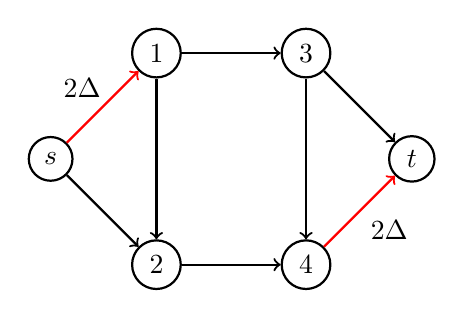
\begin{tikzpicture}[node distance={19mm}, thick , main/.style = {draw, circle}] 
    % Disegna i nodi del grafo
    
    \node[main] (0) {$s$};
    \node[main] (1) [above right of = 0] {1};
    \node[main] (2) [below right of = 0] {2};
    \node[main] (3) [right of = 1] {3};
    \node[main] (4) [right of = 2] {4};
    \node[main] (5) [below right of = 3] {$t$};
    
    \draw[->] (0) [red] to (1);
    \draw[->] (1) to (3);
    \draw[->] (0) to (2);
    \draw[->] (2) to (4);
    \draw[->] (3) to (5);
    \draw[->] (4) [red] to (5);
    \draw[->] (1) to (2);
    \draw[->] (3) to (4);

    \node at (0.4,0.9) {$2\Delta$};
    \node at (4.3,-0.9) {$2\Delta$};

\end{tikzpicture}&\begin{tikzpicture}
    \node {$\implies$};% Freccia verso destra
    \node at (0,1.4) {};
    \node at (0,-1.6) {};
\end{tikzpicture}  &
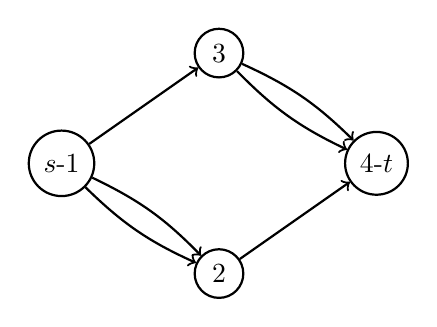
\begin{tikzpicture}[node distance={19mm}, thick , main/.style = {draw, circle}] 
    % Disegna i nodi del grafo
    \node[main] (0) {$s$-$1$};
    \node[main] (3) at (2,1.4) {$3$};
    \node[main] (2) at (2,-1.4) {$2$};
    \node[main] (4) at (4,0) {4-$t$};

    \draw[->] (0) to (3);
    \draw[->] (0) [bend left = 10] to (2);
    \draw[->] (0) [bend right = 10] to (2);
    
    
    \draw[->] (2) to (4);
    \draw[->] (3) [bend left = 10] to (4);
    \draw[->] (3) [bend right = 10] to (4);
    

\end{tikzpicture}
\end{tabular}\]

And so all the abundant cycles

\[\begin{tabular}{ccc}
    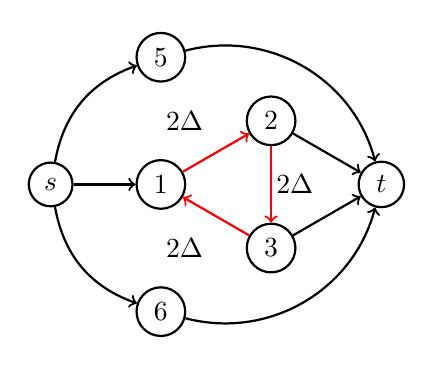
\begin{tikzpicture}[node distance={18mm}, thick , main/.style = {draw, circle}] 
    % Disegna i nodi del grafo
    
    \node[main] (0) {$s$};
    \node[main] (1) at (1*1.4,0) {1};
    \node[main] (2) at (2*1.4,0.577*1.4) {2};
    \node[main] (3) at (2*1.4,-0.577*1.4) {3};
    \node[main] (4) at (3*1.4,0) {$t$};
    \node[main] (5) at (1*1.4,1.154*1.4) {$5$};
    \node[main] (6) at (1*1.4,-1.154*1.4) {$6$};

    \draw[->] (0) [bend left] to (5);
    \draw[->] (0) [bend right] to (6);
    \draw[->] (0)  to (1);
    \draw[->] (1)[red]  to (2);
    \draw[->] (2)[red]  to (3);
    \draw[->] (3)[red]  to (1);
    \draw[->] (2)  to (4);
    \draw[->] (3)  to (4);
    \draw[->] (5) [bend left = 45] to (4);
    \draw[->] (6) [bend right = 45] to (4);

    \node at (3.1,0) {$2\Delta$};
    \node at (1.7,0.577*1.4) {$2\Delta$};
    \node at (1.7,-0.577*1.4) {$2\Delta$};
    

\end{tikzpicture}&\begin{tikzpicture}
    \node {$\implies$};% Freccia verso destra
    \node at (0,1.4) {};
    \node at (0,-1.6) {};
\end{tikzpicture}  &
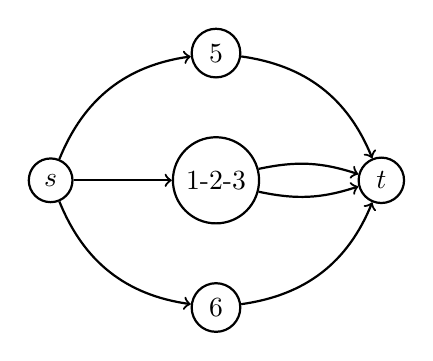
\begin{tikzpicture}[node distance={19mm}, thick , main/.style = {draw, circle}] 
    % Disegna i nodi del grafo
    \node[main] (0) {$s$};
    \node[main] (1) at (1.5*1.4,0) {1-2-3};
    \node[main] (5) at (1.5*1.4,1.154*1.4) {$5$};
    \node[main] (6) at (1.5*1.4,-1.154*1.4) {$6$};
    \node[main] (4) at (3*1.4,0) {$t$};

    \draw[->] (0) [bend left] to (5);
    \draw[->] (5) [bend left] to (4);
    \draw[->] (0) [bend right] to (6);
    \draw[->] (6) [bend right] to (4);

    \draw[->] (0) to (1);
    \draw[->] (1) [bend left= 15] to (4);
    \draw[->] (1) [bend right = 15] to (4);

\end{tikzpicture}
\end{tabular}\]

\begin{obs}
    It is possible that when the contracted graph is expanded again, the flow conservation law may be violated.
\end{obs}
    However, this violation is minor, at most \(2\Delta\) units; thus, as shown by Goldberg and Rao, the contraction, expansion, and adjustment for flow conservation can be performed in \(O(m)\) time.

\section{How to compact network}

In addition to the contraction of the graph, another transformation is necessary: the \textit{compaction}. To obtain a compact graph, we first demonstrate how to achieve an intermediate version, namely the \textbf{strongly compact network}.

It is important to understand the difference between contracting and compacting:

In contraction, a single node is created that represents the abundant cycle, and the original edges not belonging to the cycle are preserved. However, when compacting a graph, a node that has all adjacent edges abundant is \underline{eliminated}, and the outgoing edges are consequently replaced by pseudo-edges.
\[\begin{tabular}{ccc}
    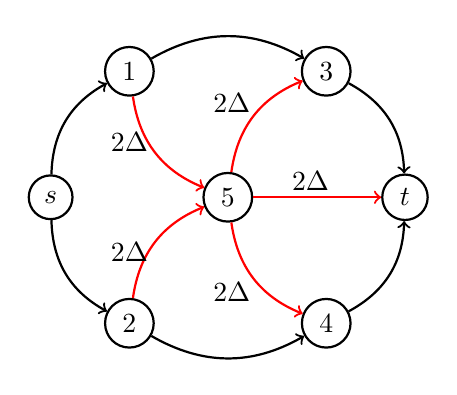
\begin{tikzpicture}[node distance={18mm}, thick , main/.style = {draw, circle}] 
    % Disegna i nodi del grafo
    
    \node[main] (0) {$s$};
    \node[main] (1) at (1, 1.6) {1};
    \node[main] (2) at (1, -1.6) {2};
    \node[main] (3) at (3.5, 1.6) {3};
    \node[main] (4) at (3.5, -1.6) {4};
    \node[main] (6) at (2.25,0) {5};
    \node[main] (5) at (4.5, 0) {$t$};

    \draw[->] (0)[bend left] to (1);
    \draw[->] (0)[bend right] to (2);
    \draw[->] (1)[bend left] to (3);
    \draw[->] (2)[bend right] to (4);
    \draw[->] (4)[bend right] to (5);
    \draw[->] (3)[bend left] to (5);

    \draw[->] (1)[red, bend right] to (6);
    \draw[->] (6)[red, bend right] to (4);
    \draw[->] (6)[red, bend left] to (3);
    \draw[->] (2)[red, bend left] to (6);
    \draw[->] (6) [red] to (5);

    \node at (3.3,0.2) {$2\Delta$};
    \node at (2.3,1.2) {$2\Delta$};
    \node at (2.3,-1.2) {$2\Delta$};

    \node at (1,.7) {$2\Delta$};
    \node at (1,-.7) {$2\Delta$};
    

\end{tikzpicture}&\begin{tikzpicture}
    \node {$\implies$};% Freccia verso destra
    \node at (0,1.4) {};
    \node at (0,-1.95) {};
\end{tikzpicture}  &
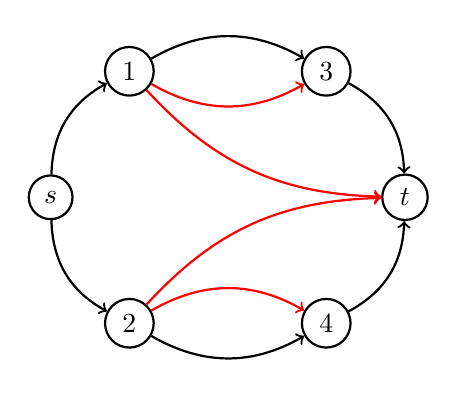
\begin{tikzpicture}[node distance={19mm}, thick , main/.style = {draw, circle}] 
    % Disegna i nodi del grafo
    \node[main] (0) {$s$};
    \node[main] (1) at (1, 1.6) {1};
    \node[main] (2) at (1, -1.6) {2};
    \node[main] (3) at (3.5, 1.6) {3};
    \node[main] (4) at (3.5, -1.6) {4};
    \node[main] (5) at (4.5, 0) {$t$};

    \draw[->] (0)[bend left] to (1);
    \draw[->] (0)[bend right] to (2);
    \draw[->] (1)[bend left] to (3);
    \draw[->] (2)[bend right] to (4);
    \draw[->] (4)[bend right] to (5);
    \draw[->] (3)[bend left] to (5);

    \draw[->] (1)[red, bend right] to (3);
    \draw[->] (2)[red, bend left] to (4);
    \draw[->] (2)[red, bend left = 23] to (5);
    \draw[->] (1)[red, bend right = 23] to (5);


\end{tikzpicture}
\end{tabular}\]

The following algorithm has a time complexity of \(O(m + |E^{sc}|)\) since pseudo-edges can be constructed in \(O(1)\) time, given that the transitive closure is dynamically preserved.

\begin{definition}[Strongly compact network]

    We define the \textbf{Strongly compact} as \(G^{sc} =(N^{sc}, E^{sc})\) originated from the network \(G\):
    \begin{enumerate}
        \item Contract the graph of all abundant cycles and the external abundant edges.\\
        Let \((r,S,T)\) be the input after contraction.
        \item Let \(N^{sc}\subseteq N(G)\) be the set of nodes that are adjacent to at least one non-abundant edge.\\
        We will refer to \(N(G)\setminus N^{sc}\) as the set of \textit{strongly compactible} nodes.
        \item We define the edges as \(E^{sc} = E^1 \cup E^2\) where:\\
        \(E^1 = \{(i,j): i\in N^{sc}\land j\in N^{sc}\land (i,j)\in E(G)\}\)\\
        \(E^2 = \{(i,j): i\in N^{sc}\land j\in N^{sc}\land i\implies j\}\)\\
        Thus, we have original edges in \(E^1\) and pseudo-edges that derive from the abundant paths.
    \end{enumerate}
\end{definition}

When we contract the graph, we are sure that if the flow routed in the contracted graph is less than a certain parameter \(\Delta\) with which we contracted the graph, then that flow is also adaptable on the original one. The following theorem shows us that the same is true for strongly compact graphs.
\newpage

\begin{theorem}[$f_{max} = f_{max}^{sc}$]

    \label{fmaxfsc}
    Let \(f_{max}\) be the maximum flow in the network \(G\) and let \(f_{max}^{sc}\) be the maximum flow in \(G^{sc}\). Then 
    \[f_{max} = f_{max}^{sc}\]
\end{theorem}

\begin{proof}
    We have already shown that any flow in \(G^{sc}\) can be rerouted in \(G\).
    If we take a flow in \(G\), it can be routed in \(G^{sc}\) using the \textbf{flow decomposition} to obtain from \(f\) a set of paths that differ by at least one edge,
    \[f := \{P^0, P^1, ..., P^k\}\]
    We can further subdivide each \(P^a\in f\) into subpaths \[P^{a}_{i\rightarrow j}| i\in N^{sc}\land j\in N^{sc}\land \forall q \in P^a_{i\rightarrow j}, q\not = i \land q\not = j \implies q\in N\setminus N^{sc}\] 
    At this point, we replace each \(P^{a}_{i\rightarrow j}\) in \(G\) that is not entirely contained in \(G^{sc}\) with the corresponding pseudo-edge \((i,j)\).

\end{proof}



\section{From sc-compact to $\Gamma$-compact}
An sc-compact graph is not sufficiently compacted for our purpose, so it will be further compacted. To avoid confusion, we will use another parameter for this additional compaction.

The second parameter is \(\Gamma\).  
The \(\Gamma\)-compact graph (composed solely of \(\Gamma\)-critical nodes) is formed starting from the sc-compact network and transferring capacities from paths where the only \(\Gamma\)-critical nodes are the endpoints, to pseudo-edges that connect these endpoints.

The parameter \(\Gamma\) is also used to ensure that in each improvement phase, there are always "enough" nodes. Thus, \(\Gamma\) initially takes the same value as \(\Delta\), but if, in a given improvement phase, the \(\Gamma\)-critical nodes are too few, a smaller \(\Gamma\) will be chosen to increase their number.

The definition of "enough" nodes and how the value of \(\Gamma\) is selected will be shown later.

Before proceeding, it’s important to distinguish between different types of edges.
\begin{definition}[Capacity Classifications]
    An edge $(i,j)$ with respect to \gmm\ has:
    \begin{enumerate}
        \item \textbf{small capacity} if $u_{ij}+u_{ji} < \Gamma/(64m^3)$
        \item \label{media}\textbf{medium capacity} if $\Gamma/(64m^3) \le u_{ij}+u_{ji}\ \land r_{ij} < 2\Delta \land r_{ji} < 2\Delta $
        \item \textbf{abundant capacity} if $r_{ij} \ge 2\Delta$ 
        \item \textbf{anti-abundant capacity} if $(j,i) \in E^{ab} \lor\ (i,j)$ is a non-abundant external edge.
    \end{enumerate}
    Where $E^{ab}$ and $E^{-ab}$ represent, respectively, the set of abundant and anti-abundant edges at the beginning of the improvement phase.

   
    
\end{definition}
\begin{obs}
    Since we have contracted abundant cycles, \[(i,j)\in E^{ab}\implies (j,i)\not \in E^{ab}\]
\end{obs}


Another necessary tool to decide which nodes to compact is the \textbf{potential function}.
\begin{definition}[Potential function]

    Given a node $j\in N$, a residual capacity function $r$, and a subset of edges adjacent to $j$ $(\tilde{E}(j))$  we can define the potential function as:
    \[\Phi (j, r, \tilde{E}(j)) = \sum_{(i,j)\in \tilde{E}(j)} r_{ij}-\sum_{(j,i)\in \tilde{E}(j)} r_{ji}\] 
\end{definition}

Based on these parameters, in each improvement phase, nodes that can be compacted are distinguished from those that cannot. These two distinctions are referred to as \gmm-compactible nodes and \gmm-critical nodes respectively.
    \begin{definition}[$\Gamma$-critical e $\Gamma$-compactible]
        
        A node $j$ is said to be \gmm-critical if it is adjacent to at least one \gmm-medium edge or if  $|\Phi (j, r, E^{-ab})| > \Gamma/(16m^2)$.

        If a node is not \gmm-critical, then it is said to be \textbf{\gmm-compactible}.

        
        Given a network $G$, we define the \textbf{\gmm-compact network} of $G$ as: \[G^c := (N^c, E^c)\]
        where $N^c$ consists of all and only \gmm-critical nodes, while $E^c$ is the set of edges that will be defined later.
    \end{definition}
    To build the \gmm-compact network, units of residual capacity are iteratively transferred from various paths to pseudo-edges. The idea is to transfer capacity from paths connecting two nodes $i,j\in N$ to the edge (or pseudo-edge) $(i,j)$, allowing further compaction of the graph.
    However, these pseudo-edges are only part of the edges comprising $E^c$, which can be defined as:
    \[E^c = E^1\cup E^2 \cup E^3\]
    $E^1 = \{(i,j) | i,j\in N^c \land (i,j) \in E(G)\}$ meaning the original edges connecting two \gmm-critical nodes.\\
    $E^2 = \{(i,j) | i,j\in N^c \land i\implies j\}$, i.e., the abundant edges.

    The edges in $E^3$ are the pseudo-edges created by transferring flow from paths consisting of anti-abundant edges. The following lemma shows that, if selected based on an appropriate criterion, the flow transfer does not reduce the capacity of any (S, T) cut, thus preserving the maximum flow that can be computed.
    \begin{lemma}[Flow transfer safety]
        \label{ftsafe}

        Let \((S,T)\) be an s-t cut in \(G\) with \(r(S,T) \leq \Delta\), and let \(A' = E^{-ab}\).  
        Suppose there exists \(P \subseteq A'\), a path from \(i \rightarrow j\), and that \((i,j) \in A'\).  
        If \(r'\) is the new residual capacity function obtained by shifting \(\delta\) units of residual capacity from \(P\) to \((i,j)\), then we can state that:

        \begin{enumerate}
            \item $\forall k\in N(G),\ \Phi(k,r',A') = \Phi(k,r,A') $
            \item $r'(S,T) = r(S,T)$
        \end{enumerate}
        
    \end{lemma}
    \begin{proof}
        Let's divide the proof by points:
        \begin{enumerate}
            \item The first point is intuitive because, for each node in $P$ that is different from $i$ and $j$, I am subtracting the same residual capacity for both incoming and outgoing edges, while for nodes $i$ and $j$, the summations of $\Phi$ remain unchanged.
            \item The second point is trivial if $|P|= 1$, so let's consider the case where $|P|\ge 2$. Define $P = p_1, ..., p_k$,where $p_1 \in S$ and at least one $p_q\in T$.\\
            Since we have established that $r(S,T) \le \Delta$ and $P\subseteq A'$ we are definitely in a situation like this:
                \[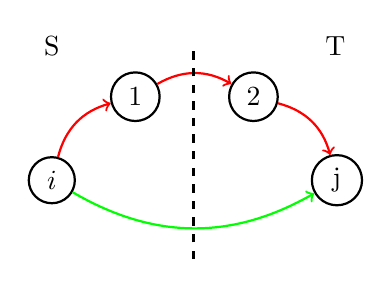
\begin{tikzpicture}[node distance={15mm}, thick , main/.style = {draw, circle}] 
                    % Disegna i nodi del grafo
                    \node[main] (0) {$i$};
                    \node[main] (1) [above right of = 0] {1};
                    \node[main] (2) [right of = 1] {2};
                    \node[main] (3) [below right of = 2] {j};
                    \node at (0,1.7) {S};
                    \node at (3.6,1.7) {T};

                    \draw[->] (0) [red, bend left] to (1);
                    \draw[->] (1) [red, bend left] to (2);
                    \draw[->] (2) [red, bend left] to (3);
                    \draw[->] (0) [green, bend right] to (3);

                    \draw[dashed] (1.8,-1) -- (1.8,1.7);
                \end{tikzpicture}\]
                Because if an edge of $P$ passed from T to S, it would violate $r(S,T)\le \Delta$ since $\forall (a,b)\in A'(\Delta),\ r_{ab} < 2\Delta \land r_{ba}\ge 2\Delta$, we would have:
                \[\begin{tikzpicture}[node distance={15mm}, thick , main/.style = {draw, circle}] 
                    % Disegna i nodi del grafo
                    \node[main] (0) {$i$};
                    \node[main] (1) [above right of = 0] {1};
                    \node[main] (2) at (3.8,0) {2};
                    \node[main] (3) [below right of = 0] {j};
                    \node at (0,1.7) {S};
                    \node at (3.6,1.7) {T};

                    \draw[->] (0) [red,bend left] to (1);
                    \draw[->] (1) [red,bend left] to (2);
                    \draw[->] (2) [red,bend left] to (3);
                    \draw[->] (3) [thick = 1.5, darktangerine, bend left] to (2);
                    \draw[->] (0) [green, bend right] to (3);

                    \draw[dashed] (1.8,-1.7) -- (1.8,1.7);
                    \node at (2.4, -.4) {\text{\color{darktangerine}{$2\Delta$}}};
                \end{tikzpicture}\]
                So the $(S,T)$ would have certainly a residual capaciti $\ge \Delta$.
                Once this has been established, it becomes clear that the transfer of residual capacity does not affect the residual capacity of the cut.
        \end{enumerate}
    \end{proof}
    We can then observe the following:

    \begin{definition}[Transferrable residual capacity]
    
    To transfer $\delta$ capacity from a path \( P \) from \( i \rightarrow j \) to the arc \( (i,j) \), the following conditions must be satisfied:
    \begin{enumerate}
        \item \( |P| \ge 2 \)
        \item \( r(P) > 0 \)
        \item \( P \subseteq A' \)
    \end{enumerate}
    
    Moreover, when creating the \(\Gamma\)-compact network, the following additional conditions are essential:
    \begin{enumerate}
        \item \( i,j \in N^c \)
        \item \( P \setminus \{i,j\} \subseteq N(G) \setminus N^c \)
    \end{enumerate}
    
    \end{definition}
    
    The capacity transferred from \( P \) is given by:
    \[
    \delta = r(P) = \min_{(a,b) \in P} r(a,b)
    \]
    Thus, each time, at least one anti-abundant arc is saturated. If there exists a path \( P \subseteq A' \) from \( i \rightarrow j \) but \( (i,j) \notin E(G) \), a pseudo-arc is created. These are the anti-abundant pseudo-arcs that will form \( E^3 \).
    
    We now analyze the procedure to transfer all residual capacities needed to form \( E^3 \) and return the set of arcs with their respective residual capacities \( r^c_{ij} \) for every \( (i,j) \in E^3 \).
    
    The algorithm takes as input (in addition to the residual function \( r \)) the set of \(\Gamma\)-critical nodes and the set of anti-abundant arcs that do not connect two \(\Gamma\)-critical nodes:
    \begin{itemize}
        \item \( G^c := \{n \mid n \in N(G) \land \Gamma\text{-critical}(n)\} \)
        \item \( H := \{(i,j) \mid (i,j) \in E^{-ab} \land (i \notin G^c \lor j \notin G^c)\} \)
    \end{itemize}
    
\begin{algorithm}
    \caption{\textit{capacity-transfer(r, H, $G^c$)}}
    \label{algotrans}
    \begin{algorithmic}[1]
     
        \For{$(i,j)\in H$} 
            \State $q_{ij} = r_{ij}$
        \EndFor
        \While{H $\not = \varnothing$}
            \State pick $i\ |\ \exists (i,k)\in H \land\nexists (j,i) \in H$
            \State pick $l\ |\ l\in N^c \lor \nexists (l,k)\in H$
            \State P = $DFS(i, l)$ \Comment{use DFS to find a path from $i$ to $l$}
            \State \(\delta = \min_{(a,b)\in P}q_{ab}\)
            \If{$i,l \in N^c$} 
                \State $A^3 = A^3 \cup {(i,l)}$
                \State $r^c_{il} $\verb|+=|$ \delta$
            \EndIf
            \For{$(a,b) \in P$}
                \State  $q_{ab} $\verb|-=|$ \delta$
            \EndFor
            \State $H = H\setminus \{(a,b) | q_{ab} = 0\}$ 
        \EndWhile 
        \Return $H, r$ 
    \end{algorithmic}
\end{algorithm}

In step 6, a path from the selected node \( i \) to a node \( l \) is created using a **depth-first search**, satisfying specific requirements. It's important to note that it \textbf{is not guaranteed} that \( i \) and \( l \) are \(\Gamma\)-critical, meaning that this path (which always exists) might be discarded.

When a path is discarded, we say that \(\delta\) capacity has been \textbf{lost}. Thus, the maximum flow in the \(\Gamma\)-compact graph is lower than the optimal one. However, the following lemma shows that there is an upper bound to this lost residual capacity.

\begin{lemma}[Bound on lost capacity in \(\Gamma\)-compact] \label{boundlose}
    Let \( f_{max} \) be the maximum flow computed in \( G \), the original network, and let \( f^* \) be the flow computed in \( G^c \), the compacted network created by the \nameref{algotrans}.
    Then:
    \[
    f^* \leq f_{max} \leq f^* + \frac{\Gamma}{16m}
    \]
    meaning that the maximum flow computed in \( G^c \) is underestimated by at most \( \frac{\Gamma}{16m} \).
\end{lemma}

\begin{proof}
    For a path to be discarded, it must start or end at a \(\Gamma\)-compactible node, that is, a node \( j \) not adjacent to a medium arc such that:
    \[
    |\Phi(j, r, E^{-ab})| = \left| \sum_{(i,j) \in E^{-ab}} r_{ij} - \sum_{(j,i) \in E^{-ab}} r_{ji} \right| \leq \frac{\Gamma}{16m^2}
    \]
    However, for a non-critical node to be chosen, it must have only incoming or only outgoing arcs, depending on which end of the path we are discussing.
    
    We can estimate that the maximum capacity of a discarded path \( P_s \) is:
    \[
    r(P_s) \leq \frac{\Gamma}{16m^2}
    \]
    which represents the maximum residual value achievable by an arc at one of the path's ends.
    
    Given that there can be at most \( n \) such paths, we have:
    \[
    n \cdot \frac{\Gamma}{16m^2} \leq m \cdot \frac{\Gamma}{16m^2} = \frac{\Gamma}{16m}
    \]
    Therefore, the maximum capacity lost in creating \( G^c \) is precisely \( \Gamma/16m \).
\end{proof}

We now need to ensure that a flow computed in \( G^c \), which we will call \(\alpha\)-optimal, can be transferred back to the original network \( G \).

Let \( f' \) be the flow computed in \( G^c \), and let \( f \) represent the transposition of \( f' \) in \( G \):
\begin{itemize}
    \item If \( f'_{i,j} > 0 \) and \( (i,j) \in E(G) \), then \( f_{i,j} = f'_{i,j} \), meaning it can be directly applied without modification.
    \item If \( f'_{i,j} > 0 \) and \( i \Rightarrow j \), it represents the compaction of an abundant path, and to restore the flow, we can use the transitivity matrix.
\end{itemize}

  
The most interesting case occurs when we need to transfer the flow from a pseudo-arc of abundant edges back to the paths that generated it. It is important to recall that the capacity of the pseudo-arc is the sum of the residual capacities of the paths that were previously transferred.

Tracking all transferred paths would be too inefficient; however, by using dynamic trees, we can enhance the algorithm previously used to keep a record of all operations performed on the tree. This way, by consulting the record backward, we can reconstruct in time \( k\log n \) (where \( k \) is the number of operations on the link-cut tree) the capacities transferred during the procedure, thereby adjusting the correct portion of flow for each edge.

Let’s now study the adaptation from the perspective of the \((S,T)\)-cut:

Let \((S',T')\) be a cut in \( G[r] \), and suppose there are no abundant edges from \( S \) to \( T \).  
A cut \((S^c, T^c)\) in \( G^c \) is said to be \textbf{induced by} \((S', T')\) if:
\[
(S^c, T^c) := (S' \cap N(G^c),\ T' \cap N(G^c))
\]
In other words, \( S^c \) is the intersection of \( S' \) with the set of nodes in \( G^c \), and similarly for \( T^c \).

Conversely, a cut in \( G^c \) is said to be induced by one in \( G[r] \) if composed as follows:

\begin{obs}
    We observe that if a cut \((S',T')\) is induced by \((S^c,T^c)\), then \((S^c,T^c)\) is also induced by \((S',T')\).
    \[
    (S',T')\leftarrow(S^c,T^c)\implies (S^c,T^c)\leftarrow(S',T')
    \]

    The reverse is not true, as different cuts on \( G[r] \) can induce the same \((S^c,T^c)\).
\end{obs}

\begin{lemma}
    Suppose \((S',T')\) is a cut in \( G[r] \) and there are no abundant edges from \( S \) to \( T \). If \((S^c,T^c)\) is induced by \((S',T')\), then
    \[
    r(S^c,T^c) \leq r(S',T') \leq r(S^c,T^c) + \Gamma / 16m
    \]
\end{lemma}

\begin{proof}
    We know that the original edges in \( E^1 \) contribute equally in both \((S^c,T^c)\) and \((S',T')\). The abundant edges are absent by hypothesis, leaving only those in \( E^3 \).
    
    We divide the paths computed by the \nameref{algotrans} into \( P \cup Q \), where \( Q \) are those that are eventually discarded.
    From \cref{ftsafe}, we know that transferring capacity does not affect the cut capacity. Therefore, the only edges that can influence the residual capacity are those in \( Q \).
    
    But from \cref{boundlose}, we know that:
    \[
    \sum_{p \in Q} r(p) \leq \Gamma / 16m
    \]
\end{proof}

From the previous lemmas, we can assert the following theorem:

\begin{theorem}
    Let \( y \) be an \(\alpha\)-optimal flow in the \gmm-compact network \( G^c \).
    Let \((S^c, T^c)\) be a cut in \( G^c \) such that \[ r(S^c, T^c) \leq val(y) + \alpha. \]
    If \((S', T')\) is the cut induced by \((S^c, T^c)\) in \( G[r] \) and \( y' \) is the respective flow, then
    \[
    val(y') = val(y).
    \]
    Moreover, \( y' \) is said to be \(\alpha'\)-optimal, where \(\alpha' = \alpha + \Gamma / 16m\).\\
    Therefore, \( r(S', T') \leq v + \alpha'. \)
\end{theorem}


\section{Max flow in $O(nm)$ time}

In this section, we will demonstrate how it is possible to compute the max flow in time \( O(nm) \) when \( m = O(n^{1.06}) \) (Note: \( 16/15 = 1.0\bar{6} \)). We will also show that the bottleneck of this procedure is due to maintaining the transitive closure of \( G^{ab} \).

\begin{algorithm}
\caption{\textit{Improve-approx-2(r,S,T)}}
\label{imp2}
\begin{algorithmic}[1]
\State $\Delta := r(S,T)$
\State $c = |N^c|$
\If{$c \ge m^{9/16}$}
    \State $\Gamma = \Delta$
    \State find a $\Gamma/(8m)$-optimal flow in $G[r]$
\ElsIf{$m^{1/3}\le c \le m^{9/16}$}
    \State $\Gamma = \Delta$
    \State $G^c:= \Gamma$-compact network
    \State $y=\Gamma/(8m)$-optimal flow in $G^c$
    \State $y' = induced(y, G[r])$
    \State $update(r)$
\ElsIf{$c<m^{1/3}$}
    $\Gamma = choseGamma(c, \Delta)$
    \State $G^c:= \Gamma$-compact network
    \State $y=$ optimal flow in $G^c$
    \State $y' = induced(y, G[r])$
    \State $update(r)$
\EndIf
\end{algorithmic}
\end{algorithm}

One of the first things we can understand by observing this algorithm is the complexity required for the creation of the \gmm-compact network, which we state in the following theorem.

\begin{theorem}[Constructing a compact network]
    \label{tgcomp}
    Suppose the algorithm dynamically maintains the transitive closure of the abundance graph and that the \gmm\ parameter is provided initially. Then, the algorithm takes \( O(m^{9/8}) \) time to create the compact graph \( G^c \).
\end{theorem}

\begin{proof}
    To contract the connected abundant components, as well as cycles, takes \( O(m) \) time. Regarding the compacted graph:
    \begin{itemize}
        \item The edges in \( E^1 \) can be calculated in \( O(m) \);
        \item The edges in \( E^3 \) can be calculated in \( O(m \log m) \) using dynamic trees;
        \item The most complex to calculate are the abundant edges in \( E^2 \), which are determined based on the transitive closure that requires a cost of \( |N^c|^2 \) to maintain.
    \end{itemize}
    However, the algorithm constructs \( G^c \) only if the number of \gmm-critical nodes is less than \( m^{9/16} \), thus the cost becomes
    \[
    O((m^{9/16})^2) = O(m^{9/8}).
    \]
\end{proof}


To demonstrate that the overall complexity of the algorithm is indeed as stated initially, we need to establish bounds both on the actions performed and the objects analyzed. The first thing to declare is that the total number of all \gmm-critical nodes analyzed during the various phases is \( O(m) \).

\begin{theorem}[Max critical node in \( O(m) \)]
    \label{maxM}
    Suppose that each improvement phase meets the required conditions; then the \gmm-critical nodes calculated during the iterations total \( O(m) \).
\end{theorem}

\begin{proof}
    For a node \( j \) to be \gmm-critical, it must be adjacent to a \gmm medium edge, or it must not have adjacent \gmm medium edges but have \( |\Phi (j, r, E^{-ab})| > \Gamma/(16m^2) \), i.e., it must be \gmm-special.

    First, consider the nodes adjacent to a \gmm-medium edge:\\
    \textbf{Claim:}
    An edge can have medium \gmm-capacity for at most 3 consecutive phases.

    \textit{Proof:}
    Let \( (i,j) \) be an edge with \gmm-medium capacity, then \( u_{ij} + u_{ji} \ge \Gamma/64m^3 \). Given that in each phase \( \Delta' = \frac{\Delta}{8m} \), in the immediate next phase, we have 
    \[
    u_{ij} + u_{ji} \ge \Gamma/64m^3 \ge \Delta'/8m^2 = \Delta''/m = 8\Delta'''
    \]
    Thus, after 3 phases, \( u_{ij} + u_{ji} \ge 8\Delta \), implying that either \( (i,j) \) or \( (j,i) \) has become abundant, and the edge is no longer \gmm-medium. \QED

    For the other \gmm-special edges:\\
    \textbf{Claim:}
    Let \gmm\ be the compactness parameter of a given \dlt-improvement phase, and let \( j \) be a \gmm-special node. If \( \Delta^* \) is the bound 4 phases after \dlt, then there exists a node \( k \) such that 
    \[
    r_{jk} \ge 2\Delta^* \quad \text{and} \quad r_{kj} \ge 2\Delta^* 
    \]
    implying that \( (j,k) \) (and also \( (k,j) \)) is \textit{doubly-abundant}, and thus will be contracted.
    
    \textit{Proof:}\\
    First, define \( v^* \) as the flow in phase \( \Delta^* \) such that \( r^* = r_{ij}-v_{ij}+v_{ji} \). From lemma \ref{ab4ever}, we know that every \dlt-abundant edge will also be \( \Delta^* \)-abundant. Furthermore,
    \[
    r_{ij}^* > \Gamma/64m^3 \implies r_{ij}^* > 8\Delta^*
    \]

    Suppose there exists an abundant edge \( (j,k) \) with \( v_{jk}^* > \Gamma/64m^3 \); then for the opposite edge \( (k,j) \), we have:
    \[
    r^*_{k,j}= r_{kj}-v^*_{kj}+r^*_{jk}> 8\Delta^*
    \]
    Thus, the opposite is also \( \Delta^* \)-abundant, and the nodes \( j \) and \( k \) will be contracted.

    It remains to check the case where a node \( j \) is \gmm-special without having abundant edges with flow greater than \( \Gamma/64m^3 \).\\
    We know that:
    \[
    |\Phi (j, r, E^{-ab})| = |\hat{r}_{out}(j)-\hat{r_{in}}(j)|> \Gamma/(16m^2)
    \]
    Consider the case where \( \hat{r}_{out}(j)-\hat{r_{in}}(j)> \Gamma/(16m^2) \) (the other case is similar). We have:
    \[
    \sum_{j:(j,k)\in E^{-ab}}y^*_{jk} \le \sum_{j:(j,k)\in E}y^*_{jk} = \sum_{j:(i,j)\in E}y^*_{ij}
    \]
    due to flow conservation. Furthermore, 
    \[
    \sum_{j:(i,j)\in E}y^*_{ij} < \sum_{j:(i,j)\in E^{-ab}}y^*_{ij} + \sum_{j:(i,j)\in E^{ab}}y^*_{ij}+ m\Gamma/64m^3
    \]
    But since we have assumed that no abundant edge has flow greater than \( \Gamma/64m^3 \),
    \[
    \begin{array}{rl}
        < & \hat{r}_{in}(j) + 2m\Gamma/64m^3\\
        < & (\hat{r}_{out}(j) - \Gamma/16m^2) + \Gamma/32m^2\\
        < & \hat{r}_{out}(j) - \Gamma/32m^2\\
        = & \sum_{j:(j,k)\in E^{-ab}}r_{jk} - \Gamma/32m^2
    \end{array}
    \]

    Thus, there must exist some edge for which 
    \[
    y^*_{jk}<r_{jk}-\Gamma/32m^3 \implies r^*_{jk}\ge r_{jk}-y^*_{jk}>\Gamma/32m^3>16\Delta^*
    \]
    Therefore, there exists some \( (j,k) \) non-abundant edge in the \dlt phase that becomes abundant in the phase \( \Delta^* \), and since \( (k,j) \) is also abundant, the cycle will be contracted. \QED

    We have shown through the two claims that all \gmm-critical nodes in a phase cannot remain \gmm-critical for more than a constant number of consecutive phases. The fact that they have a "limited duration" and are at most \( O(m) \) proves the statement.
\end{proof}

Knowing the number of nodes to analyze, the next step is to estimate the number of \textbf{improvement phases} required to calculate the maximum flow. However, it is necessary first to understand how the \gmm\ parameter is chosen.
\newpage
\begin{lemma}[\gmm\ Parameter]
    \label{gammchose}
    The \gmm\ parameter can be chosen in \( O(m+n\log n) \) time.
\end{lemma}

\begin{proof}
    We give a procedure that does this: 
    \begin{enumerate}
        \item For each node \( j \), calculate the largest \gmm' value for which \( j \) is \gmm'-critical (\textit{time required} \( O(m) \)).
        \item Order the nodes \( j \) by their \gmm' value (\textit{time required} \( O(n\log n) \)).
        \item Choose the \gmm\ value such that there are at most \( m^{1/3} \) nodes \( j \) with \( \Gamma'(j) \ge \Gamma \) (\textit{time required} \( O(1) \)).
    \end{enumerate}
\end{proof}

We now have all the tools to calculate the number of improvement phases:

\begin{lemma}
    The number of improvement phases is \( O(m^{2/3}) \).
\end{lemma}

\begin{proof}
    From theorem \ref{maxM}, we know that the number of \gmm-critical nodes analyzed is \( O(m) \), and from lemma \ref{gammchose}, we know that in each improvement phase at least \( m^{1/3} \) nodes are analyzed.

    When we demonstrated that the number of nodes was \( O(m) \), the proof relied on the fact that the nodes had a "deadline" and would be contracted in at most 3 or 4 consecutive phases. Thus, all at least \( m^{1/3} \) nodes analyzed in one phase will be "consumed" in \( O(1) \) phases.

    Consequently, the number of phases required to "consume" them all is \( O(m^{2/3}) \).
\end{proof}

From the following lemmas, we can derive the total time required to create all the \( G^c \).

\begin{lemma}
    The total time to create all the compact networks is \( O(nm + m^{43/24}) \).
\end{lemma}
\begin{proof}
    We know that the \gmm\ parameter requires time \( O(m + n \log n) \).\\
    We know that creating a compact network takes \( O(m^{9/8}) \) time.\\
    Since the number of phases is \( O(m^{2/3}) \),\\
    putting everything together, we obtain:
    \[ O(mn + m^{43/24}) \]
\end{proof}

Finding a flow that is \(\alpha\)-optimal means finding a flow that is at most \(\alpha\) less than the maximum capacity flow. We have seen that if we search for the maximum flow in the \gmm-compact network \( G^c \) and then transfer it to the original network \( G \), this is already \(\Gamma/16m\)-optimal.

However, during the algorithm, we aim to obtain this approximation directly in \( G \). If we recall the functioning of the Goldberg-Rao algorithm, we can see that the algorithm terminates when its estimate of the maximum flow is less than 1. By intervening on this maximum flow estimate, it is possible to terminate the algorithm before reaching the optimal flow, resulting in a gap of at most a value of \(\alpha\) of our choosing.

Now let’s reason about the cost \( T \) of a phase of the Goldberg-Rao algorithm, knowing that we are executing it on a graph with \( C \) nodes and \( O(C^2) \) edges.
\[ \Lambda = O(C^{2/3}), \quad T = \tilde{O}(C^{2/3} \cdot C^2) = \tilde{O}(C^{8/3}) \]

We can now evaluate the cost of the \nameref{imp2} procedure.

Moreover, we can note that if we execute the Goldberg-Rao algorithm on a total of \( O(m) \) nodes while performing a maximum of \( \log U \) phases, the average number of nodes in each improvement phase is
\[ C = O\left( \frac{m}{\log{U}} \right) \]
This is the reason why we construct the compact graph only if \( C \le m^{9/16} \). In fact, if the Goldberg algorithm is polynomial, then if \( \log U \le m^{7/16} \):
\[ C \ge m^{9/16} \implies \frac{m}{\log U} \ge m^{9/16} \implies \log U \le \frac{m}{m^{9/16}} = m^{7/16} \]


\begin{lemma}[Time of improve-max]
    The time to compute the optimal flow using the \textit{improve-approx-2} procedure is 
    \[ O(m^{31/16} \log^2 m) \]
\end{lemma}
\begin{proof}
    Given that a total of \( O(m) \) \gmm-critical nodes are computed, I will calculate the cost of the procedure for a single node rather than for the number of phases:
    
    Let \( T \) be the time required to find an \(\alpha\)-optimal flow.\\
    We know that if \( C \ge m^{9/16} \), we can find an optimal flow with \( T = O(m^{3/2} \log^2 n) \) by executing \( \log n \) phases of the Goldberg-Rao algorithm on the original graph. When scaled to the number of \gmm-critical nodes, we have \( T/C = m^{15/16} \log^2 n \).
    
    If instead \( m^{1/3} \le C < m^{9/16} \), we work in the compact graph and seek the maximum flow, executing \( \log n \) phases of the Goldberg-Rao algorithm, thus \( T = O(C^{8/3} \log n) \). Therefore, 
    \[ T/C = O(m^{5/3} \log n = m^{15/16}) \].
    
    Finally, if \( C < m^{1/3} \), the small number of edges leads the cost to be \( T = O(C^3) \), resulting in \( T/C = O(C^2) = O(m^{2/3}) \).

    We can assert that in every case, the cost of the procedure for each node is \( O(m^{15/16} \log^2 n) \). Multiplying this result by the number of \gmm-critical nodes across all increments yields 
    \[ O(m \cdot m^{15/16} \log^2 n) = O(m^{31/16} \log^2 n) \]. 
\end{proof}

\begin{lemma}
    The total time to transform all the flows computed on \( G^c \) into flows on the residual graph is 
    \[ O(nm + m^{5/3} \log n) \].
\end{lemma}
\begin{proof}
    Let \( G^c \) be the compact graph derived from \( G[r] \) (the residual graph), and let \( y^c \) be the flow in \( G^c \) while \( y \) is the flow induced on the residual graph.

    The edges of \( G^c \) are divided into three categories: \( E^c = E^1 \cup E^2 \cup E^3 \), corresponding to original edges, abundant pseudo-edges, and anti-abundant pseudo-edges.

    For any edge \( (i,j) \) such that \( y^c_{ij} > 0 \), we distinguish the three cases:
    \begin{enumerate}
        \item If \( (i,j) \in E^1 \implies y_{ij} = y^c_{ij} \).
        \item If \( (i,j) \in E^2 \), we know that to reconstruct the abundant path we need \( O(|P|) = O(n) \). Furthermore, by utilizing dynamic trees, we can keep the number of edges with positive flow in \( E^2 \) below the value \( C \) at a cost of \( O(m \log n) \), repeated for \( O(m^{2/3}) \) phases, resulting in \( O(m^{5/3} \log n) \). In this way, all abundant paths are restored in \( O(nm) \). We always remember that the cost of dynamically maintaining the transitive closure is \( O(nm) \).
        \item Regarding the edges in \( E^3 \), we again have to resort to dynamic trees to reconstruct the anti-abundant paths that we contracted. Specifically, it is not possible to keep track of all paths efficiently; however, we can maintain a record of all operations performed on the graph to retrace and restore the old paths. This procedure also has a total cost of \( O(m \log n \cdot m^{2/3}) \). 
    \end{enumerate}
    
    We conclude that the total time to induce the flow in \( G^c \) to \( G[r] \) for all \( m^{2/3} \) phases is 
    \[ O(nm + m^{5/3} \log n) \]
\end{proof}

From the previous lemmas, we can deduce the following theorem:

\begin{theorem}[Max flow in \( O(nm) \)]
    If the flow in each improvement phase is computed using the \textit{improve-approx-2} procedure, then the time to find the maximum flow is 
    \[ O(nm + m^{31/16} \log^2 n) \]
    If \( m = O(n^{1.06}) \), the running time is $O(nm)$.
\end{theorem}


\cleardoublepage